\chapter{अभिक्रिया की एन्थैल्पी}\label{ch:b2:reaction-enthalpy}

एक छोटे बर्नर के नीचे कसा हुआ कैंपिंग-गैस का कारतूस: कुछ ग्राम ब्यूटेन एक
लीटर पानी को मिनटों में उबाल देती है, और बर्तन के नीचे की नीली ज्वाला उबलते
पानी से कहीं अधिक गर्म होती है। कोई अभिक्रिया कितनी ऊष्मा मुक्त करती है, उसमें
से कितनी बर्तन तक पहुँचती है, और ज्वाला कितनी गर्म हो सकती है? इनमें से किसी भी
प्रश्न का उत्तर पाने के लिए बर्नर की आवश्यकता नहीं: प्रति पदार्थ कुछ संख्याओं की
सारणियाँ, जो एक बार सदा के लिए मापी गई हैं, उन पदार्थों से लिखी जा सकने वाली
हर अभिक्रिया की ऊष्मा किसी भी ताप पर दे देती हैं। यह अध्याय वही लेखा-जोखा
खड़ा करता है। यह भौतिकी से ज्ञात ऊष्मागतिकी के प्रथम नियम को ऐसे निकाय पर
लागू करता है जिसका संघटन बदलता है, अभिक्रिया की एन्थैल्पी को एक आंशिक अवकलज के
रूप में परिभाषित करता है, और दिखाता है कि उसे संभवन एन्थैल्पियों से, आबंध
एन्थैल्पियों से और चक्रों के अनुदिश कैसे परिकलित करें, ताप के साथ वह कैसे
बदलती है, और ज्वालाओं तथा कैलोरीमीटरों के बारे में वह क्या बताती है।

\begin{recall}
भौतिकी से: प्रथम नियम $\Delta U = W + Q$; एन्थैल्पी $H = U + pV$, जो एक
अवस्था फलन है; स्थिर बाह्य दाब पर, उसी दाब की दो अवस्थाओं के बीच, प्राप्त
ऊष्मा $Q_p = \Delta H$ है; स्थिर दाब पर ऊष्मा धारिता
$C_p = (\partial H/\partial T)_p$ है; आदर्श
गैस की एन्थैल्पी केवल $T$ पर निर्भर करती है। प्रथम वर्ष के खंड ने अभिक्रियारत
निकाय का वर्णन उसकी प्रगति $\xi$ और
रससमीकरणमितीय संख्याओं $\nu_i$ से किया था, जो $0 = \sum_i\nu_i\mathrm A_i$ की हैं,
और हर स्पीशीज़ की मानक अवस्था $p^\circ = \qty{1}{bar}$ पर नियत की थी। विद्यालय
के खंड (कक्षा 11) ने ऊष्मा मुक्त करने वाली अभिक्रिया को \omterm{def:b2:reaction-enthalpy:exothermic}{ऊष्माक्षेपी} कहा था और
आबंध ऊर्जाओं से दहन ऊर्जाओं का आकलन किया था।
\end{recall}

\begin{omfigure}
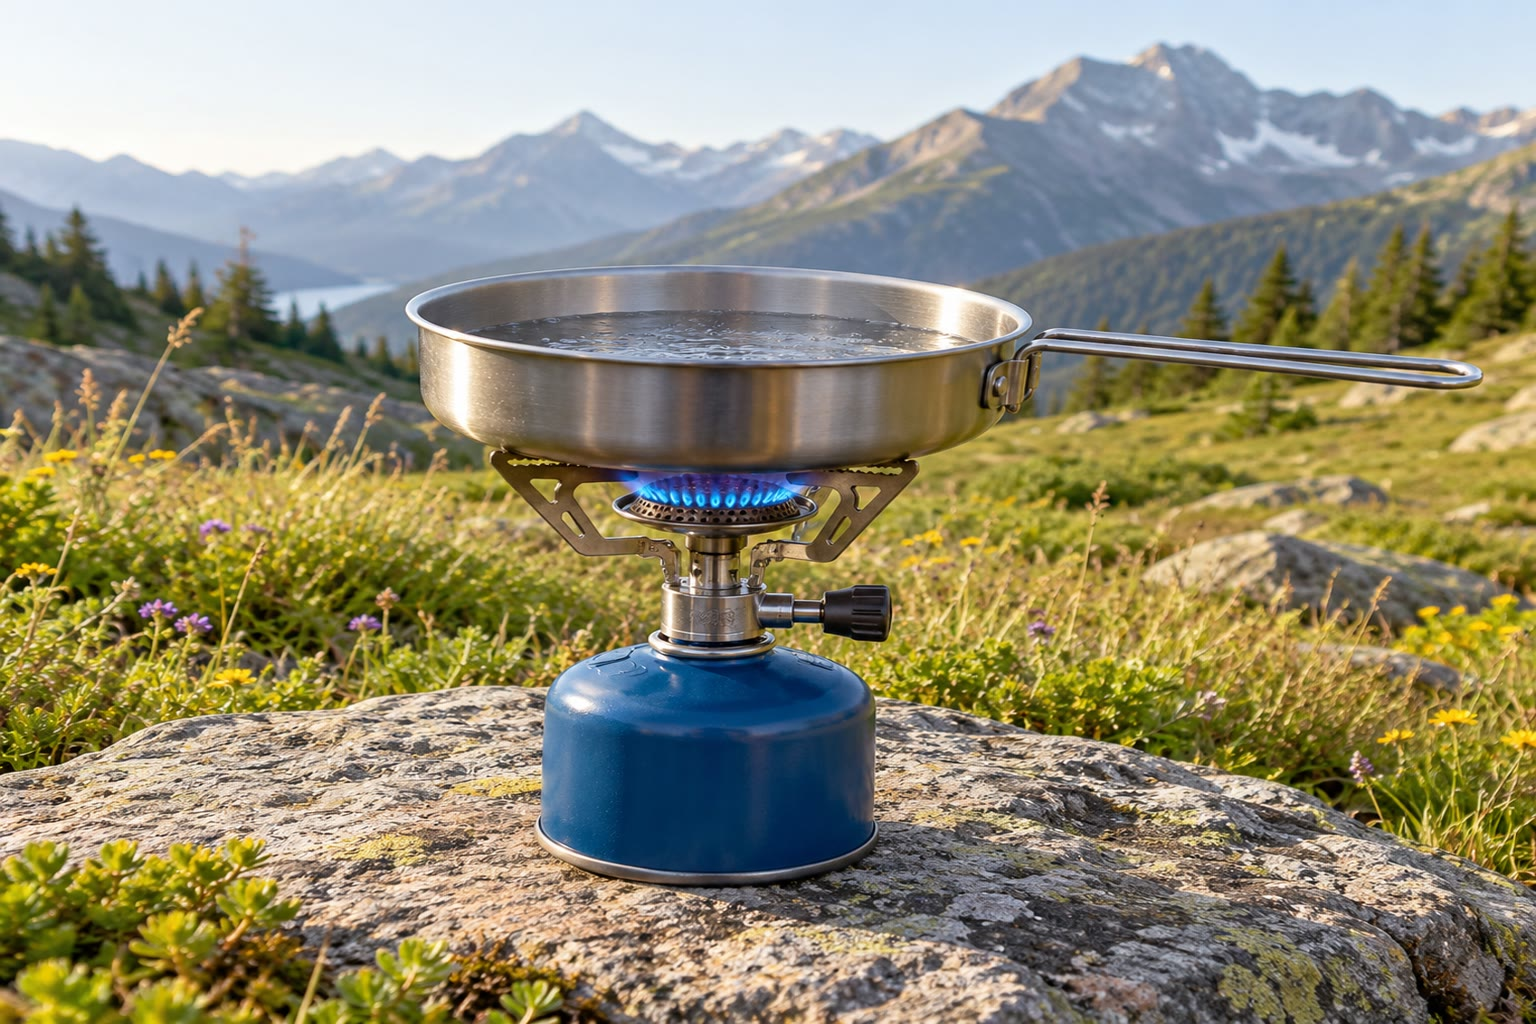
\includegraphics[width=0.6\linewidth]{images/book3/ai/b2-01-camping-stove.jpg}

{\small कैंपिंग स्टोव: कारतूस की ब्यूटेन बर्तन के नीचे वायु में जलती है। प्रति
मोल ब्यूटेन मुक्त ऊष्मा, उसका वह अंश जो पानी तक पहुँचता है, और ज्वाला का
ताप इस अध्याय की सप्ताहांत समस्या में परिकलित किए
गए हैं।}
\end{omfigure}

\section{अभिक्रिया राशियाँ}

जिस बंद निकाय में केवल एक अभिक्रिया $0 = \sum_i\nu_i\mathrm A_i$
होती है, उसका वर्णन उसके ताप, दाब और प्रगति से होता है:
मात्राएँ $n_i = n_{i,0} + \nu_i\xi$ हैं। तब निकाय का हर विस्तीर्ण अवस्था फलन,
उदाहरण के लिए उसकी एन्थैल्पी, एक फलन $H(T, p,
\xi)$ है, और उसका यथातथ अवकल यह है:
\[
  \dd H = \left(\frac{\partial H}{\partial T}\right)_{p,\xi}\dd T
        + \left(\frac{\partial H}{\partial p}\right)_{T,\xi}\dd p
        + \left(\frac{\partial H}{\partial \xi}\right)_{T,p}\dd\xi .
\]

\begin{definition}[अभिक्रिया राशि, अभिक्रिया एन्थैल्पी]\label{def:b2:reaction-enthalpy:reaction-quantity}
ऐसे बंद निकाय के किसी विस्तीर्ण अवस्था फलन $X$ के लिए, जिसमें
अभिक्रिया $0 = \sum_i\nu_i\mathrm A_i$ होती है, \emph{अभिक्रिया
राशि}\index{अभिक्रिया राशि} यह आंशिक अवकलज है:
\[
  \Delta_r X = \left(\frac{\partial X}{\partial \xi}\right)_{T,p} ,
\]
अर्थात् नियत ताप और दाब पर प्रति इकाई प्रगति $X$ का परिवर्तन, जिसका मात्रक
$X$ का मात्रक प्रति मोल है। $X = H$ के लिए यह \emph{अभिक्रिया
एन्थैल्पी}\index{अभिक्रिया एन्थैल्पी} $\Delta_r H$ है, \unit{kJ/mol} में।
\end{definition}

\begin{remark}[अवकलज, अंतर नहीं]\label{rem:b2:reaction-enthalpy:operator}
प्रतीक $\Delta_r$ एक संकारक है: यह निकाय की अवस्था पर लगता है, और उसे
अपरिवर्तित छोड़ता है। अभिक्रिया को दूसरे ढंग से लिखने पर (उसके गुणांक दुगुने
करने पर) $\Delta_r H$ दुगुना हो जाता है, इसलिए अपने समीकरण के बिना \omterm{def:b2:reaction-enthalpy:reaction-quantity}{अभिक्रिया
राशि} का कोई अर्थ नहीं। जब स्पीशीज़ की आंशिक मोलर एन्थैल्पियाँ
$\bar H_i = (\partial H/\partial n_i)_{T,p,n_j}$ प्रयुक्त होती हैं
(\cref{ch:b2:chemical-potential}), तब $\Delta_r H = \sum_i\nu_i\bar H_i$, जो
$n_i = n_{i,0} + \nu_i\xi$ पर शृंखला नियम लगाने से मिलता है।
\end{remark}

\begin{proposition}[नियत ताप और दाब पर प्राप्त ऊष्मा]\label{prop:b2:reaction-enthalpy:qp}
जब अभिक्रिया $\xi_1$ से $\xi_2$ तक आगे बढ़ती है, और निकाय नियत $T$
और $p$ पर रखा जाता है, तो निकाय यह ऊष्मा प्राप्त करता है:
\[
  Q_p = \int_{\xi_1}^{\xi_2}\Delta_r H\,\dd\xi = \Delta_r H\,(\xi_2 - \xi_1)
\]
जब $\Delta_r H$, $\xi$ पर निर्भर नहीं करता।
\end{proposition}

\begin{proof}
नियत $p$ पर (और, यहाँ, नियत बाह्य दाब पर) प्राप्त ऊष्मा एन्थैल्पी
का परिवर्तन है, $Q_p = \Delta H$ (भौतिकी)। नियत $T$ और $p$ पर
$H$ का अवकल घटकर $\dd H = \Delta_r H\,\dd\xi$ रह जाता है; $\xi_1$ से
$\xi_2$ तक समाकलन करने पर परिणाम मिलता है।
\end{proof}

\begin{definition}[ऊष्माक्षेपी, ऊष्माशोषी, ऊष्मा-उदासीन]\label{def:b2:reaction-enthalpy:exothermic}
कोई अभिक्रिया किसी दी गई अवस्था में \emph{ऊष्माक्षेपी}\index{ऊष्माक्षेपी} है यदि
$\Delta_r H < 0$: नियत $T$ और $p$ पर अग्र दिशा में चलने पर वह परिवेश को
ऊष्मा देती है। वह \emph{ऊष्माशोषी}\index{ऊष्माशोषी} है यदि $\Delta_r H >
0$, और \emph{ऊष्मा-उदासीन}\index{ऊष्मा-उदासीन} यदि $\Delta_r H = 0$।
\end{definition}

अभिक्रिया की ऊष्मा सामान्यतः संघटन पर निर्भर नहीं करती:
आदर्श गैसों और शुद्ध ठोसों व द्रवों के लिए हर स्पीशीज़ की
एन्थैल्पी इस पर निर्भर नहीं करती कि उसके आसपास क्या है, और $\Delta_r H$
का मान $T$ नियत होते ही नियत हो जाता है।

\begin{proposition}[आदर्श निकाय]\label{prop:b2:reaction-enthalpy:ideal}
शुद्ध संघनित प्रावस्थाओं सहित आदर्श गैसों के मिश्रण में $\Delta_r H$
केवल ताप पर निर्भर करता है, और नीचे परिभाषित \omterm{def:b2:reaction-enthalpy:standard-reaction-enthalpy}{मानक अभिक्रिया
एन्थैल्पी} $\Delta_r H^\circ(T)$ के बराबर होता है। तनु विलयन के
विलेयों के लिए यह समता अच्छे सन्निकटन तक सत्य है।
\end{proposition}

\begin{proof}
आदर्श-गैस मिश्रण में हर गैस ऐसे व्यवहार करती है मानो अकेली हो, और उसकी
एन्थैल्पी $n_iH_{m,i}(T)$ होती है जो $p$ पर निर्भर नहीं करती (भौतिकी: आदर्श
गैस की एन्थैल्पी केवल $T$ पर निर्भर करती है)। शुद्ध ठोस या द्रव के लिए $H = n_iH_{m,i}(T,
p)$, और संघनित प्रावस्था के लिए $(\partial H_m/\partial p)_T = V_m(1 - \alpha T)$ कुछ
\unit{J/(mol.bar)} ही है, जो दसियों \unit{kJ/mol} की \omterm{def:b2:reaction-enthalpy:reaction-quantity}{अभिक्रिया
एन्थैल्पियों} की तुलना में नगण्य है। अतः $H = \sum_in_iH_{m,i}(T)$, जिसका
$\xi$ के सापेक्ष अवकलज $\sum_i\nu_iH_{m,i}(T)$ है: यह केवल
$T$ पर निर्भर करता है, और इसका मान वही है जो हर स्पीशीज़ को उसकी
मानक अवस्था में लेकर परिकलित होता है।
\end{proof}

\section{मानक अभिक्रिया एन्थैल्पियाँ और हेस का नियम}

\begin{definition}[मानक अभिक्रिया राशि]\label{def:b2:reaction-enthalpy:standard-reaction-enthalpy}
\emph{मानक अभिक्रिया राशि}\index{मानक अभिक्रिया राशि}
$\Delta_r X^\circ(T) = \sum_i\nu_iX_{m,i}^\circ(T)$ वह \omterm{def:b2:reaction-enthalpy:reaction-quantity}{अभिक्रिया राशि} है
जो ताप $T$ पर हर स्पीशीज़ को उसकी मानक अवस्था में लेकर परिकलित होती है,
$X_{m,i}^\circ$ मानक मोलर मान हैं। $X = H$ के लिए यह
\emph{मानक अभिक्रिया एन्थैल्पी}\index{मानक अभिक्रिया एन्थैल्पी}
$\Delta_r H^\circ(T)$ है; यह केवल $T$ पर निर्भर करती है।
\end{definition}

केवल एन्थैल्पी के अंतर ही मापे जा सकते हैं, इसलिए एक संदर्भ सदा के लिए चुन
लिया जाता है, जैसे विभवों के लिए हाइड्रोजन इलेक्ट्रोड चुना गया था।

\begin{definition}[मानक संदर्भ अवस्था, मानक संभवन एन्थैल्पी]\label{def:b2:reaction-enthalpy:formation}
ताप $T$ पर किसी तत्व की \emph{मानक संदर्भ अवस्था}\index{मानक संदर्भ अवस्था}
ताप $T$ पर, $p^\circ$ के अंतर्गत, उसका सबसे स्थायी रूप है:
\ce{H2}, \ce{O2}, \ce{N2} और \ce{Cl2} आदर्श गैसों के रूप में, कार्बन
ग्रेफ़ाइट के रूप में, सोडियम धातु के रूप में, ब्रोमीन द्रव के रूप में (\qty{298}{K} पर)।
किसी यौगिक की \emph{मानक संभवन एन्थैल्पी}\index{मानक संभवन एन्थैल्पी}
$\Delta_f H^\circ$ उसकी संभवन अभिक्रिया की \omterm{def:b2:reaction-enthalpy:standard-reaction-enthalpy}{मानक अभिक्रिया
एन्थैल्पी} है, अर्थात् उस अभिक्रिया की जो यौगिक का एक मोल उसके
तत्वों से, उनकी संदर्भ अवस्थाओं में, बनाती है। रचना से ही,
संदर्भ अवस्था वाले तत्व के लिए $\Delta_f H^\circ = 0$।
\end{definition}

\begin{example}[संभवन अभिक्रियाएँ]\label{ex:b2:reaction-enthalpy:formation}
जल की संभवन अभिक्रिया \ce{H2(g) + 1/2O2(g) -> H2O(l)} है,
\qty{298.15}{K} पर $\Delta_f H^\circ = \qty{-285.83}{kJ/mol}$ के साथ;
मेथेन की \ce{C(s) + 2H2(g) -> CH4(g)} है, $\Delta_f H^\circ =
\qty{-74.9}{kJ/mol}$; नाइट्रोजन मोनॉक्साइड की, \ce{1/2N2(g) + 1/2O2(g) ->
NO(g)}, $\Delta_f H^\circ = \qty{+90.3}{kJ/mol}$: एक \omterm{def:b2:reaction-enthalpy:exothermic}{ऊष्माशोषी} यौगिक,
जिसे इंजन की गर्म गैसें फिर भी बना देती हैं। आधे गुणांक कोई समस्या
नहीं हैं: संभवन अभिक्रिया लेखा-जोखे का एक साधन है, कोई
क्रियाविधि नहीं।
% ledger: dfh:H2O-l, dfh:CH4_g, dfh:NO_g
\end{example}

\begin{theorem}[हेस का नियम]\label{thm:b2:reaction-enthalpy:hess}
यदि कोई अभिक्रिया, गुणांकों $\lambda_k$ के साथ, अभिक्रियाओं $k$ का योग है,
तो उसकी \omterm{def:b2:reaction-enthalpy:standard-reaction-enthalpy}{मानक अभिक्रिया एन्थैल्पी} उनकी एन्थैल्पियों का वही संयोजन है:
$\Delta_r H^\circ = \sum_k\lambda_k\Delta_r H_k^\circ$
(\emph{हेस का नियम}\index{हेस का नियम})। विशेष रूप से, \omterm{def:b2:reaction-enthalpy:standard-reaction-enthalpy}{मानक अभिक्रिया एन्थैल्पी}
अभिक्रियाओं के किसी भी ऐसे पथ के अनुदिश परिकलित की जा सकती है जो
अभिकारकों से उत्पादों तक ले जाए।
\end{theorem}

\begin{proof}
हर $\Delta_r H_k^\circ = \sum_i\nu_{i,k}H_{m,i}^\circ$ रससमीकरणमितीय
संख्याओं में रैखिक है। यदि अभिक्रिया, भारित योग $\sum_k\lambda_k$ के रूप में,
अभिक्रियाओं $k$ से बनी है, तो उसकी रससमीकरणमितीय संख्याएँ $\nu_i = \sum_k\lambda_k
\nu_{i,k}$ हैं, और $\Delta_r H^\circ = \sum_i\nu_iH_{m,i}^\circ = \sum_k\lambda_k
\sum_i\nu_{i,k}H_{m,i}^\circ$। इस बीजगणित के पीछे प्रथम नियम है: $H$ एक
अवस्था फलन है, इसलिए समान प्रारंभिक और अंतिम अवस्थाओं के बीच उसका परिवर्तन
पथ पर निर्भर नहीं करता।
\end{proof}

\begin{proposition}[संभवन एन्थैल्पियों से अभिक्रिया एन्थैल्पी]\label{prop:b2:reaction-enthalpy:formation-sum}
$\Delta_r H^\circ(T) = \sum_i\nu_i\,\Delta_f H_i^\circ(T)$.
\end{proposition}

\begin{proof}\emergencystretch=3em
वह पथ लीजिए जो अभिकारकों को उनकी संदर्भ अवस्थाओं वाले तत्वों में
विघटित करता है (उनकी संभवन अभिक्रियाओं का उलटा, गुणांकों
$-\nu_i > 0$ के साथ), फिर उन्हीं तत्वों से उत्पाद बनाता है
(गुणांक $\nu_i > 0$)। समीकरण संतुलित है, इसलिए तत्व कट जाते हैं,
और \omterm{thm:b2:reaction-enthalpy:hess}{हेस का नियम} एन्थैल्पियों को जोड़ देता है।
\end{proof}

\begin{omfigure}
\begin{tikzpicture}[font=\small, >={Stealth}, y=0.0062cm]
  \draw[->] (0,-1000) -- (0,180) node[above] {$H^\circ$ (\unit{kJ/mol})};
  \foreach \y in {0,-200,-400,-600,-800,-1000} \draw (-0.08,\y) -- (0.08,\y) node[left=4pt] {$\y$};
  % levels
  \draw[very thick] (1.0,0) -- (4.6,0) node[right] {\ce{C(s) + 2H2(g) + 2O2(g)}};
  \draw[very thick, omDef] (1.0,-74.9) -- (4.6,-74.9);
  \node[right, omDef] at (4.6,-110) {\ce{CH4(g) + 2O2(g)}};
  \draw[very thick, omThm] (1.0,-965.2) -- (4.6,-965.2) node[right] {\ce{CO2(g) + 2H2O(l)}};
  % arrows
  \draw[->, omDef, thick] (1.6,0) -- (1.6,-74.9);
  \node[omDef, anchor=south west, font=\footnotesize] at (1.1,5) {$\Delta_f H^\circ(\ce{CH4}) = -74.9$};
  \draw[->, omThm, thick] (3.9,0) -- (3.9,-965.2);
  \node[right, omThm, align=left] at (3.95,-500) {$\Delta_f H^\circ(\ce{CO2})$\\ $+ 2\Delta_f H^\circ(\ce{H2O})$\\ $= -965.2$};
  \draw[->, thick] (2.75,-74.9) -- (2.75,-965.2);
  \node[left, align=right] at (2.7,-650) {$\Delta_r H^\circ$\\ $= -890.3$};
\end{tikzpicture}

{\small \qty{298.15}{K} पर मेथेन के दहन के एन्थैल्पी स्तर।
संदर्भ अवस्थाओं वाले तत्व शून्य हैं। मेथेन उनसे
\qty{74.9}{kJ/mol} नीचे है, उत्पाद \qty{965.2}{kJ/mol} नीचे:
दहन एन्थैल्पी इनका अंतर, \qty{-890.3}{kJ/mol}, है, ज्वाला वास्तव में
चाहे जिस पथ से चले।}
% ledger: dfh:CH4_g, dfh:CO2, dfh:H2O-l
\end{omfigure}

\begin{example}[मेथेन का दहन]\label{ex:b2:reaction-enthalpy:methane}\emergencystretch=3em
\ce{CH4(g) + 2O2(g) -> CO2(g) + 2H2O(l)} के लिए,
\qty{298.15}{K} पर $\Delta_r H^\circ = -393.51 + 2(-285.83) - (-74.87) - 0 =
\qty{-890.3}{kJ/mol}$। कैलोरीमीटर में मापा गया मान
\qty{-890.7}{kJ/mol} है: सारणी और ज्वाला आँकड़ों की अनिश्चितता के भीतर
सहमत हैं। यदि जल वाष्प के रूप में निकले
($\Delta_f H^\circ = \qty{-241.83}{kJ/mol}$), तो $\Delta_r H^\circ =
\qty{-802.3}{kJ/mol}$: अंतर, \qty{88.0}{kJ}, दो मोल जल के वाष्पन की
एन्थैल्पी है, जिसे गैस बॉयलर अपने धुएँ को संघनित करके
पुनः प्राप्त करता है।
% ledger: dfh:CO2, dfh:H2O-l, dfh:CH4_g, dch:CH4, dfh:H2O_g (computed in figdata/bachelor-2/thermo-data.py)
\end{example}

\begin{method}[हेस चक्र]\label{met:b2:reaction-enthalpy:hess-cycle}
ऐसी अभिक्रिया की एन्थैल्पी ज्ञात करने के लिए जो सीधे मापी नहीं जा सकती:
\begin{enumerate}
  \item लक्ष्य अभिक्रिया को उसकी अवस्थाओं सहित लिखिए;
  \item ज्ञात एन्थैल्पी वाली ऐसी अभिक्रियाएँ (दहन, संभवन) खोजिए जिनका
        संयोजन, गुणांकों $\lambda_k$ के साथ, लक्ष्य देता हो;
  \item जाँचिए कि लक्ष्य में न आने वाली हर स्पीशीज़ कट जाती है;
  \item एन्थैल्पियों को उन्हीं गुणांकों से जोड़िए।
\end{enumerate}
\end{method}

\begin{example}[कार्बन से कार्बन मोनॉक्साइड]\label{ex:b2:reaction-enthalpy:co}
कार्बन को जलाने पर सदा कुछ कार्बन डाइऑक्साइड बनती है, इसलिए
\ce{C(s) + 1/2O2(g) -> CO(g)} की एन्थैल्पी सीधे नहीं मापी जाती। दोनों दहन
\ce{C(s) + O2(g) -> CO2(g)} ($\qty{-393.51}{kJ/mol}$) और \ce{CO(g) +
1/2O2(g) -> CO2(g)} ($\qty{-283.0}{kJ/mol}$, मापा गया) मापे जाते हैं; लक्ष्य
पहले में से दूसरे को घटाना है: $\Delta_r H^\circ = -393.51 + 283.0 =
\qty{-110.5}{kJ/mol}$, जो कार्बन मोनॉक्साइड की संभवन एन्थैल्पी है।
% ledger: dfh:CO2, dfh:CO_g
\end{example}

\begin{history}[जर्मेन आंरी हेस]
\begin{minipage}[t]{0.2\linewidth}\vspace{0pt}
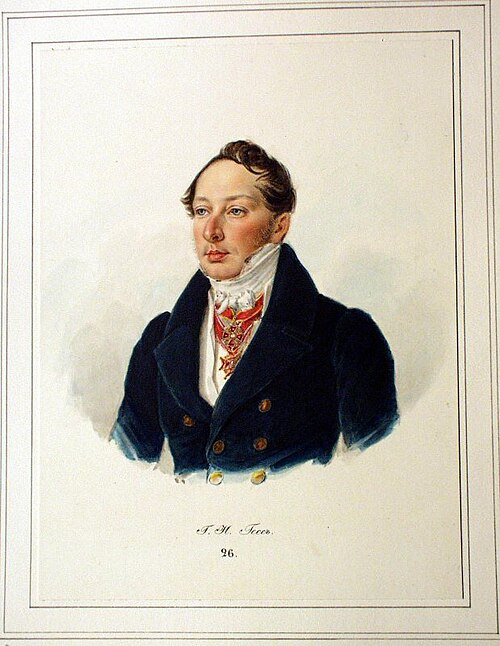
\includegraphics[width=\linewidth]{images/book3/hess.jpg}
\end{minipage}\hfill
\begin{minipage}[t]{0.76\linewidth}\vspace{0pt}
जर्मेन आंरी हेस (1802--1850), सेंट पीटर्सबर्ग में रसायन के प्राध्यापक, ने
सल्फ़्यूरिक अम्ल को कई चरणों में तनु या उदासीन करने पर मुक्त
ऊष्माएँ मापीं, और 1840 में पाया कि कुल ऊष्मा अपनाए गए चरणों पर
निर्भर नहीं करती: यह ``ऊष्मा के स्थिर योग का नियम'' था, जो
ऊष्मागतिकी के प्रथम नियम से भी पहले कहा गया, और वही नियम इसकी व्याख्या करता है।
(चित्र: इ॰ इ॰ राइमर्स, 1837--1838; CC BY-SA 4.0, विकिमीडिया कॉमन्स।)
\end{minipage}
\end{history}

\section{अभिक्रिया एन्थैल्पियों का परिकलन}

\subsection*{आबंध एन्थैल्पियों से}

जब किसी यौगिक की संभवन एन्थैल्पी उपलब्ध न हो, तो उसके आबंधों की ऊर्जा
गैस प्रावस्था में एक आकलन देती है।

\begin{definition}[आबंध वियोजन एन्थैल्पी, माध्य आबंध एन्थैल्पी]\label{def:b2:reaction-enthalpy:bond-enthalpy}
किसी गैसीय अणु में आबंध A--B की \emph{आबंध वियोजन एन्थैल्पी}\index{आबंध वियोजन एन्थैल्पी}
उस आबंध के टूटकर दो गैसीय खंडों में बदलने की \omterm{def:b2:reaction-enthalpy:standard-reaction-enthalpy}{मानक अभिक्रिया
एन्थैल्पी} है, द्विपरमाणुक अणु के लिए \ce{AB(g) -> A(g) + B(g)}।
जब किसी अणु में $n$ समान आबंध हों, तो उसकी
\emph{माध्य आबंध एन्थैल्पी}\index{माध्य आबंध एन्थैल्पी} गैसीय परमाणुओं में
उसके पूर्ण परमाणुकरण की मानक एन्थैल्पी को $n$ से भाग देने पर मिलती है।
\end{definition}

परमाणुकरण एन्थैल्पियाँ स्वयं संभवन एन्थैल्पियाँ ही हैं: गैसीय परमाणुओं की
संभवन एन्थैल्पियाँ, ऋण अणु की संभवन एन्थैल्पी। नीचे की सारणी इसी प्रकार
परिकलित की गई है।

\begin{omfigure}
\begin{tabular}{lrl}
\hline
आबंध & एन्थैल्पी (\unit{kJ/mol}) & किससे प्राप्त \\
\hline
H--H & 436 & \ce{H2}, वियोजन \\
O=O & 498 & \ce{O2}, वियोजन \\
N$\equiv$N & 945 & \ce{N2}, वियोजन \\
Cl--Cl & 243 & \ce{Cl2}, वियोजन \\
H--Cl & 432 & \ce{HCl}, वियोजन \\
C--H & 416 & \ce{CH4}, चार का माध्य \\
N--H & 391 & \ce{NH3}, तीन का माध्य \\
O--H & 464 & \ce{H2O}, दो का माध्य \\
C=O & 804 & \ce{CO2}, दो का माध्य \\
C--C & 330 & \ce{C2H6}, C--H मेथेन से लेकर \\
C=C & 589 & \ce{C2H4}, C--H मेथेन से लेकर \\
\hline
\end{tabular}

\smallskip
{\small \qty{298.15}{K} पर आबंध एन्थैल्पियाँ, गैसीय परमाणुओं और अणुओं की \omterm{def:b2:reaction-enthalpy:formation}{मानक
संभवन एन्थैल्पियों} से परिकलित। अंतिम दो
पंक्तियाँ विधि की सीमा दिखाती हैं: एथेन का C--H आबंध ठीक-ठीक मेथेन
का C--H आबंध नहीं है, और C--C का मान वह अंतर विरासत में पाता है।}
% ledger: dfh:C_g, janaf:H, dfh:O_g, dfh:N_g, janaf:Cl, janaf:HCl, dfh:CH4_g, dfh:NH3_g, dfh:H2O_g, dfh:CO2, dfh:C2H6_g, dfh:C2H4_g (computed in figdata/bachelor-2/thermo-data.py)
\end{omfigure}

\begin{proposition}[आबंध एन्थैल्पियों से आकलन]\label{prop:b2:reaction-enthalpy:bond-estimate}
गैसों के बीच अभिक्रिया के लिए,
\[
  \Delta_r H^\circ \approx \sum(\text{टूटे आबंधों की एन्थैल्पियाँ}) -
  \sum(\text{बने आबंधों की एन्थैल्पियाँ}).
\]
\end{proposition}

\begin{proof}
वह पथ अपनाइए जो हर अभिकारक का परमाणुकरण करता है (एन्थैल्पी: टूटे
आबंध) और फिर परमाणुओं से उत्पाद बनाता है (ऋण बने आबंध)। जब हर आबंध
एन्थैल्पी उसी आबंध की उसके अपने अणु में हो, तब \omterm{thm:b2:reaction-enthalpy:hess}{हेस का
नियम} योग को यथातथ बनाता है; उसे किसी दूसरे अणु के माध्य मान से बदलना ही
सन्निकटन है।
\end{proof}

\begin{example}[एथीन का हाइड्रोजनन]\label{ex:b2:reaction-enthalpy:hydrogenation}
\ce{C2H4(g) + H2(g) -> C2H6(g)} में एक C=C और एक H--H टूटते हैं और
उनकी जगह एक C--C और दो C--H बनते हैं। सारणी से: $589 + 436 - 330 - 2
\times 416 = \qty{-137}{kJ/mol}$; संभवन एन्थैल्पियों से मान
\qty{-136.3}{kJ/mol} है। यहाँ सहमति अच्छी है, क्योंकि सारणी के C--C
और C=C इन्हीं अणुओं से प्राप्त किए गए थे; सारणी के अणुओं से भिन्न
अणु के लिए 10 से \qty{30}{kJ/mol} की त्रुटि सामान्य है।
% ledger: dfh:C2H4_g, dfh:C2H6_g
\end{example}

\subsection*{जालक एन्थैल्पियाँ: बॉर्न--हाबर चक्र}

\begin{definition}[जालक एन्थैल्पी]\label{def:b2:reaction-enthalpy:lattice-enthalpy}
किसी आयनिक क्रिस्टल की \emph{जालक एन्थैल्पी}\index{जालक एन्थैल्पी}
गैसीय आयनों में उसके वियोजन की \omterm{def:b2:reaction-enthalpy:standard-reaction-enthalpy}{मानक अभिक्रिया एन्थैल्पी} है:
सोडियम क्लोराइड के लिए \ce{NaCl(s) -> Na+(g) + Cl-(g)}। यह धनात्मक होती है,
और क्रिस्टल के संसंजन को मापती है।
\end{definition}

इसे सीधे मापा नहीं जा सकता, परंतु तत्वों से होकर जाने वाला चक्र इसे
मापनीय राशियों से दे देता है: क्रिस्टल की संभवन एन्थैल्पी, तत्वों का
परमाणुकरण, धातु की आयनन ऊर्जा और अधातु की इलेक्ट्रॉन बंधुता
(दोनों प्रथम वर्ष के खंड में परिभाषित)।

\begin{omfigure}
\begin{tikzpicture}[font=\small, >={Stealth}, y=0.0058cm]
  \def\lw{5.0}
  % levels (kJ/mol relative to Na(s) + 1/2 Cl2(g))
  \draw[thick] (0,0) -- (\lw,0) node[right] {\ce{Na(s) + 1/2Cl2(g)}};
  \draw[thick] (0,107.5) -- (\lw,107.5) node[right] {\ce{Na(g) + 1/2Cl2(g)}};
  \draw[thick] (0,228.8) -- (\lw,228.8) node[right] {\ce{Na(g) + Cl(g)}};
  \draw[thick] (0,724.6) -- (\lw,724.6) node[right] {\ce{Na+(g) + e- + Cl(g)}};
  \draw[thick] (0,376.1) -- (\lw,376.1) node[right] {\ce{Na+(g) + Cl-(g)}};
  \draw[thick] (0,-411.1) -- (\lw,-411.1) node[right] {\ce{NaCl(s)}};
  % the path through the elements, on the left
  \draw[->, omDef] (0.4,0) -- (0.4,107.5);
  \node[omDef, left, font=\footnotesize] at (0.35,53) {ऊर्ध्वपातन $107.5$};
  \draw[->, omDef] (0.4,107.5) -- (0.4,228.8);
  \node[omDef, left, font=\footnotesize] at (0.35,168) {$\tfrac12$ वियोजन $121.3$};
  \draw[->, omDef] (0.4,228.8) -- (0.4,724.6);
  \node[omDef, left, font=\footnotesize] at (0.35,480) {Na का आयनन $495.8$};
  \draw[->, omThm] (1.4,724.6) -- (1.4,376.1);
  \node[omThm, right, font=\footnotesize] at (1.45,560) {इलेक्ट्रॉन-संलग्नन $-348.6$};
  \draw[->, omProp] (2.3,0) -- (2.3,-411.1);
  \node[omProp, left, font=\footnotesize] at (2.25,-205) {संभवन $-411.1$};
  % the lattice enthalpy, the only unknown
  \draw[->, thick] (3.6,-411.1) -- (3.6,376.1);
  \node[right, font=\footnotesize] at (3.65,-205) {जालक एन्थैल्पी $787$};
\end{tikzpicture}

{\small \qty{298}{K} पर सोडियम क्लोराइड का बॉर्न--हाबर चक्र
(\unit{kJ/mol})। क्रिस्टल से गैसीय आयनों तक \omterm{def:b2:reaction-enthalpy:lattice-enthalpy}{जालक एन्थैल्पी} द्वारा
ऊपर जाना, या तत्वों से होकर घूमकर जाना, एक ही स्तर तक ले जाता है:
\omterm{def:b2:reaction-enthalpy:lattice-enthalpy}{जालक एन्थैल्पी} चक्र की एकमात्र अज्ञात राशि है।}
% ledger: dfh:NaCl_cr, dfh:Na_g, janaf:Cl, ie:Na, ea:Cl
\end{omfigure}

\begin{method}[बॉर्न--हाबर चक्र]\label{met:b2:reaction-enthalpy:born-haber}
\begin{enumerate}
  \item संदर्भ अवस्थाओं वाले तत्वों से दो पथ खींचिए: एक
        क्रिस्टल तक (संभवन), एक गैसीय आयनों तक (धातु का ऊर्ध्वपातन,
        अधातु का परमाणुकरण, आयनन, इलेक्ट्रॉन-संलग्नन)।
  \item चक्र को \omterm{def:b2:reaction-enthalpy:lattice-enthalpy}{जालक एन्थैल्पी} से बंद कीजिए, क्रिस्टल से ऊपर
        गैसीय आयनों तक।
  \item लिखिए कि चक्र के चारों ओर एन्थैल्पियों का योग शून्य है, और
        अज्ञात के लिए हल कीजिए। आयनन ऊर्जाएँ और इलेक्ट्रॉन बंधुताएँ
        eV प्रति परमाणु में सारणीबद्ध होती हैं: $N_A e = \qty{96.485}{kJ/(mol.eV)}$ से गुणा कीजिए।
\end{enumerate}
\end{method}

\begin{example}[सोडियम क्लोराइड]\label{ex:b2:reaction-enthalpy:nacl}
$\Delta_{\text{जालक}}H^\circ = 411.1 + 107.5 + 121.3 + 495.8 - 348.6 =
\qty{787}{kJ/mol}$। आयनन ऊर्जा और इलेक्ट्रॉन बंधुता
\qty{0}{K} की ऊर्जाएँ हैं; \qty{298}{K} तक उनके संशोधन (हर एक के लिए $+\tfrac52RT$)
दोनों चरणों के बीच कट जाते हैं। बिंदु आवेशों वाला क्रिस्टल मॉडल
लगभग यही मान देता है, इसी कारण सोडियम क्लोराइड को आयनिक कहा जाता है।
% ledger: dfh:NaCl_cr, dfh:Na_g, janaf:Cl, ie:Na, ea:Cl (computed in figdata/bachelor-2/thermo-data.py)
\end{example}

\section{अभिक्रिया एन्थैल्पियाँ और ताप}

सारणियाँ $\Delta_f H^\circ$ को \qty{298.15}{K} पर देती हैं। रिएक्टर
\qty{700}{K} पर चलता है, ज्वाला \qty{2000}{K} पर: ताप के साथ
$\Delta_r H^\circ$ कैसे बदलता है?

\begin{theorem}[किरखॉफ़ का नियम]\label{thm:b2:reaction-enthalpy:kirchhoff}
\[
  \frac{\dd\Delta_r H^\circ}{\dd T} = \Delta_r C_p^\circ =
  \sum_i\nu_i C_{p,m,i}^\circ ,
\]
अतः $\Delta_r H^\circ(T_2) = \Delta_r H^\circ(T_1) + \int_{T_1}^{T_2}
\Delta_r C_p^\circ\,\dd T$ (\emph{किरखॉफ़ का नियम}\index{किरखॉफ़ का नियम}),
बशर्ते $T_1$ और $T_2$ के बीच अवस्था-परिवर्तन न हो।
\end{theorem}

\begin{proof}
हर स्पीशीज़ को उसकी मानक अवस्था में लेने पर $H^\circ(T, \xi) = \sum_in_i
H^\circ_{m,i}(T)$ दो चरों का ऐसा फलन है जिसके द्वितीय आंशिक
अवकलज संतत हैं; श्वार्ज़ प्रमेय से वे क्रमविनिमेय हैं:
\[
  \frac{\dd\Delta_r H^\circ}{\dd T} = \frac{\partial}{\partial T}
  \frac{\partial H^\circ}{\partial\xi} = \frac{\partial}{\partial\xi}
  \frac{\partial H^\circ}{\partial T} = \frac{\partial}{\partial\xi}
  \sum_in_iC^\circ_{p,m,i} = \sum_i\nu_iC^\circ_{p,m,i}.
\]
$T_1$ और $T_2$ के बीच समाकलन करने पर दूसरा रूप मिलता है। अंतराल के भीतर
किसी स्पीशीज़ का अवस्था-परिवर्तन उसकी संक्रमण एन्थैल्पी को, रससमीकरणमितीय
संख्या के साथ, जोड़ देता है।
\end{proof}

\begin{example}[गर्म अवस्था में अमोनिया संश्लेषण]\label{ex:b2:reaction-enthalpy:kirchhoff}
\ce{N2(g) + 3H2(g) -> 2NH3(g)} के लिए $\Delta_r H^\circ(298) =
\qty{-91.9}{kJ/mol}$ और, \qty{298}{K} की ऊष्मा धारिताओं से,
$\Delta_r C_p^\circ = 2(35.65) - 29.12 - 3(28.84) =
\qty{-44.3}{J/(K.mol)}$। इसे स्थिर मानने पर $\Delta_r
H^\circ(700) = -91.9 - 0.0443 \times 402 = \qty{-109.7}{kJ/mol}$ मिलता है। सारणियाँ,
जो ताप के साथ बढ़ती ऊष्मा धारिताओं का अनुसरण करती हैं,
\qty{-105.2}{kJ/mol} देती हैं: स्थिर-$C_p$ आकलन 4\,\% हटकर है, जो
एक पंक्ति के परिकलन के लिए उचित मूल्य है। \qty{400}{K} में \omterm{def:b2:reaction-enthalpy:reaction-quantity}{अभिक्रिया
एन्थैल्पी} लगभग सातवें भाग जितनी बदल जाती है।
% ledger: dfh:NH3_g, cp:NH3_g.298, cp:N2_g.298, cp:H2_g.298, janafdfH:NH3.700 (computed in figdata/bachelor-2/thermo-data.py)
\end{example}

\section{रुद्धोष्म अभिक्रियाएँ और ऊष्मामिति}

\subsection*{ज्वाला का ताप}

ज्वाला में अभिक्रिया तीव्र होती है और ऊष्मा को बाहर निकलने का समय नहीं मिलता:
गैसें स्वयं को गर्म कर लेती हैं।

\begin{definition}[रुद्धोष्म ज्वाला ताप]\label{def:b2:reaction-enthalpy:flame-temperature}
किसी ईंधन का \emph{रुद्धोष्म ज्वाला ताप}\index{रुद्धोष्म ज्वाला ताप}
वह ताप है जिस तक उसके पूर्ण दहन के उत्पाद पहुँचते हैं, जब अभिक्रिया
\qty{298}{K} के अभिकारकों से, नियत दाब पर और ऊष्मा के किसी
विनिमय के बिना होती है।
\end{definition}

\begin{proposition}[ज्वाला ताप का परिकलन]\label{prop:b2:reaction-enthalpy:flame}
यदि अभिक्रिया $\xi$ तक आगे बढ़ती है, $T_0$ के अभिकारकों से आरंभ करके, और अंतिम
निकाय की ऊष्मा धारिता $C_p(T)$ है, तो अंतिम ताप $T_f$ इसे संतुष्ट करता है:
\[
  \xi\,\Delta_r H^\circ(T_0) + \int_{T_0}^{T_f}C_p(T)\,\dd T = 0 .
\]
\end{proposition}

\begin{proof}
रुद्धोष्म और नियत दाब पर होने के कारण रूपांतरण के लिए $\Delta H =
Q_p = 0$। चूँकि $H$ एक अवस्था फलन है, समान प्रारंभिक और अंतिम
अवस्थाओं के बीच कोई भी पथ वही $\Delta H$ देता है। नीचे के
चित्र का पथ लीजिए: पहले $T_0$ पर अभिक्रिया, जिसमें
$\Delta H_1 = \xi\Delta_r H^\circ(T_0)$ (\cref{prop:b2:reaction-enthalpy:qp},
आदर्श व्यवहार मानकर); फिर अंतिम निकाय का $T_0$ से
$T_f$ तक तापन, $\Delta H_2 = \int C_p\,\dd T$। इनका योग शून्य है।
\end{proof}

\begin{omfigure}
\begin{tikzpicture}[font=\small, >={Stealth}]
  \draw[->] (0,0) -- (6.2,0) node[right] {प्रगति $\xi$};
  \draw[->] (0,0) -- (0,3.6) node[above] {ताप $T$};
  \fill (0.6,0.6) circle (2pt) node[below left] {अभिकारक, $T_0$};
  \fill (5.2,0.6) circle (2pt) node[below] {उत्पाद, $T_0$};
  \fill (5.2,3.0) circle (2pt) node[right] {उत्पाद, $T_f$};
  \draw[->, thick, omDef] (0.7,0.6) -- (5.1,0.6);
  \node[omDef, above, font=\footnotesize] at (3.15,0.64) {$\Delta H_1 = \xi\,\Delta_r H^\circ(T_0) < 0$};
  \draw[->, thick, omThm] (5.2,0.7) -- (5.2,2.9);
  \node[omThm, right, align=left] at (5.25,1.8) {$\Delta H_2 = \int_{T_0}^{T_f} C_p\,\dd T$};
  \draw[->, thick, dashed] (0.75,0.75) -- (5.05,2.92);
  \node[above left, align=center] at (2.6,1.75) {वास्तविक ज्वाला:\\ $\Delta H = 0$};
\end{tikzpicture}

{\small रुद्धोष्म ज्वाला (खंडित रेखा) और दो चरणों वाला
एक तुल्य पथ: नियत ताप पर अभिक्रिया, फिर उत्पादों का तापन।
चूँकि $H$ एक अवस्था फलन है, दोनों चरणों के एन्थैल्पी परिवर्तनों का योग
शून्य होता है।}
\end{omfigure}

\begin{method}[ज्वाला का ताप]\label{met:b2:reaction-enthalpy:flame-temperature}
\begin{enumerate}
  \item ईंधन के एक मोल का पूर्ण दहन लिखिए; वायु में, ऑक्सीजन के साथ आने वाली
        नाइट्रोजन और आर्गन जोड़िए (वे भी गर्म होती
        हैं); जल को वाष्प के रूप में लीजिए।
  \item प्रति मोल ईंधन $q = -\Delta_r H^\circ(T_0)$ परिकलित कीजिए।
  \item या तो उत्पादों की स्थिर ऊष्मा धारिता $C_p$ लीजिए:
        $T_f = T_0 + q/C_p$; या ऐसा $T_f$ ज्ञात कीजिए कि सारणीबद्ध
        वृद्धियों $n_i[H^\circ_{m,i}(T_f) - H^\circ_{m,i}(T_0)]$ का योग
        अंतर्वेशन द्वारा $q$ के बराबर हो।
\end{enumerate}
\end{method}

\begin{omfigure}
\begin{tikzpicture}
\begin{axis}[
  width=0.8\linewidth, height=6.2cm, xmin=300, xmax=3000, ymin=0, ymax=3200,
  axis x line=bottom, axis y line=left, xlabel={$T$ (K)},
  ylabel={उत्पादों का $H(T) - H(\qty{298}{K})$ (kJ)},
  xtick={500,1000,1500,2000,2500,3000},
  tick label style={font=\small}, label style={font=\small}, clip=false,
  legend style={font=\scriptsize, draw=none, at={(0.5,1.03)}, anchor=south}, legend columns=2]
\addplot[omDef, very thick] table[x=T, y=H] {figdata/out/bachelor-2-flame-temperature-butane.dat};
\addplot[omThm, very thick] table[x=T, y=H] {figdata/out/bachelor-2-flame-temperature-methane.dat};
\legend{1 mol ब्यूटेन वायु में, 1 mol मेथेन वायु में}
\draw[omDef, dashed] (axis cs:300,2657.6) -- (axis cs:3000,2657.6);
\node[omDef, anchor=south east, font=\scriptsize] at (axis cs:2350,2657.6) {$-\Delta_r H^\circ = \qty{2657.6}{kJ}$};
\draw[omDef, dotted] (axis cs:2401,0) -- (axis cs:2401,2657.6);
\fill[omDef] (axis cs:2401,2657.6) circle (1.5pt);
\node[omDef, anchor=north west, font=\scriptsize] at (axis cs:2420,2620) {\qty{2401}{K}};
\draw[omThm, dashed] (axis cs:300,802.3) -- (axis cs:3000,802.3);
\node[omThm, anchor=south west, font=\scriptsize] at (axis cs:320,802.3) {$-\Delta_r H^\circ = \qty{802.3}{kJ}$};
\draw[omThm, dotted] (axis cs:2329,0) -- (axis cs:2329,802.3);
\fill[omThm] (axis cs:2329,802.3) circle (1.5pt);
\node[omThm, anchor=north west, font=\scriptsize] at (axis cs:2350,760) {\qty{2329}{K}};
\end{axis}
\end{tikzpicture}

{\small एक मोल ईंधन के दहन उत्पादों (कार्बन डाइऑक्साइड, भाप, और वायु की
नाइट्रोजन और आर्गन) को \qty{298}{K} से गर्म करने के लिए आवश्यक एन्थैल्पी,
सारणीबद्ध एन्थैल्पियों से। हर वक्र अपने दहन से मुक्त ऊष्मा से
\omterm{def:b2:reaction-enthalpy:flame-temperature}{रुद्धोष्म ज्वाला ताप} पर मिलता है: ब्यूटेन के लिए लगभग
\qty{2400}{K}, मेथेन के लिए \qty{2330}{K}।}
% ledger: janafH:CO2.2400, janafH:H2O.2400, janafH:N2.2400, janafH:Ar.2400, air:N2, air:O2, air:Ar (computed in figdata/bachelor-2/flame-temperature.py)
\end{omfigure}

परिकलित ताप ऊपरी सीमाएँ हैं। लगभग \qty{2000}{K} से ऊपर
कार्बन डाइऑक्साइड और जल कार्बन मोनॉक्साइड, हाइड्रोजन, ऑक्सीजन और
मूलकों में वियोजित होने लगते हैं; ये \omterm{def:b2:reaction-enthalpy:exothermic}{ऊष्माशोषी} अभिक्रियाएँ ऊष्मा का एक भाग
वापस ले लेती हैं, और वायु में ब्यूटेन की वास्तविक ज्वाला परिकलित मान से
स्पष्टतः ठंडी होती है। शुद्ध ऑक्सीजन में गर्म करने को नाइट्रोजन नहीं होती और ज्वाला
कहीं अधिक गर्म होती है, इसीलिए वेल्डर एथाइन को वायु के बजाय ऑक्सीजन के
साथ जलाते हैं।

\subsection*{ऊष्मामिति}

\begin{proposition}[नियत आयतन और नियत दाब]\label{prop:b2:reaction-enthalpy:bomb}
इस्पात के बंद पात्र (बम कैलोरीमीटर) में मापी गई ऊष्मा $Q_V =
\Delta U$ है, और आदर्श गैसों तथा संघनित प्रावस्थाओं के लिए
\[
  \Delta_r H = \Delta_r U + \Delta\nu_{\text{गैस}}\,RT ,
\]
जहाँ $\Delta\nu_{\text{गैस}}$ गैसीय स्पीशीज़ की रससमीकरणमितीय संख्याओं का
योग है।
\end{proposition}

\begin{proof}
$H = U + pV$, और $\Delta_r H = \Delta_r U + \partial(pV)/\partial\xi$, नियत $T$ पर।
संघनित प्रावस्थाओं का $pV$ नगण्य है, और
गैसों के लिए $pV = n_{\text{गैस}}RT$, जहाँ $n_{\text{गैस}} = n_{\text{गैस},0} +
\Delta\nu_{\text{गैस}}\xi$, जिसका $\xi$ के सापेक्ष अवकलज
$\Delta\nu_{\text{गैस}}RT$ है।
\end{proof}

\begin{omfigure}
\begin{tikzpicture}[font=\small, >={Stealth}, scale=1.0]
  % outer insulated jacket
  \draw[thick, fill=gray!8] (-2.6,-0.2) rectangle (2.6,4.4);
  \draw[thick, fill=white] (-2.3,0.1) rectangle (2.3,4.1);
  % water bath
  \fill[omDef!12] (-2.3,0.1) rectangle (2.3,3.4);
  \draw[omDef!60] (-2.3,3.4) -- (2.3,3.4);
  % bomb
  \draw[very thick, fill=gray!35] (-0.75,0.5) rectangle (0.75,2.6);
  \draw[very thick, fill=gray!55] (-0.9,2.6) rectangle (0.9,2.85);
  \draw[thick] (-0.3,1.0) -- (-0.3,1.9) (0.3,1.0) -- (0.3,1.9);
  \draw[thick, fill=orange!50] (-0.3,0.95) rectangle (0.3,1.05);
  \draw[red!70!black, thick, decorate, decoration={zigzag, amplitude=1pt, segment length=3pt}] (-0.3,1.9) -- (0.3,1.9);
  % wires
  \draw (-0.3,2.85) -- (-0.3,4.7) (0.3,2.85) -- (0.3,4.7);
  % stirrer and thermometer
  \draw[thick] (1.6,0.6) -- (1.6,4.7);
  \draw[thick, fill=gray!40] (1.35,0.55) rectangle (1.85,0.75);
  \pic[transform shape] at (-1.6,0.4) {thermometer};
  % labels
  \draw (-0.75,1.6) -- (-3.3,1.6) node[left] {इस्पात का बम, \qty{30}{bar} पर \ce{O2}};
  \draw (0,1.0) -- (-3.3,0.6) node[left] {कप में नमूना};
  \draw (0,1.9) -- (-3.3,2.6) node[left] {प्रज्वलन तार};
  \draw (1.0,3.0) -- (3.3,3.0) node[right] {जल-कुंड};
  \draw (1.6,3.9) -- (3.3,4.3) node[right] {विलोडक};
  \draw (-1.6,3.4) -- (-3.3,3.6) node[left] {तापमापी};
  \draw (2.45,0.3) -- (3.3,0.5) node[right] {ऊष्मारोधी आवरण};
\end{tikzpicture}

{\small बम कैलोरीमीटर। नमूना दाब के अधीन ऑक्सीजन में नियत आयतन पर
जलता है; ऊष्मा बम और विलोडित जल में जाती है, जिसकी ताप-वृद्धि
तापमापी पर पढ़ी जाती है। कैलोरीमीटर की ऊष्मा धारिता पहले से ज्ञात
ऊर्जा वाले एक मानक को जलाकर ज्ञात की जाती है।}
\end{omfigure}

\begin{method}[ऊष्मामिति]\label{met:b2:reaction-enthalpy:calorimetry}
\begin{enumerate}
  \item अंशांकन कीजिए: ज्ञात दहन ऊर्जा वाले एक मानक का कुछ द्रव्यमान जलाइए
        (या ज्ञात विद्युत ऊर्जा प्रवाहित कीजिए), ताप-वृद्धि
        $\Delta T$ पढ़िए, और पूरे कैलोरीमीटर (जल और पात्र, उसका
        ``जल-तुल्यांक'') की ऊष्मा धारिता $C$ निकालिए।
  \item नमूना जलाइए, $\Delta T'$ पढ़िए: मुक्त ऊष्मा $C\,\Delta
        T'$ है, अतः नियत आयतन पर $\Delta_r U = -C\Delta T'/\xi$।
  \item $\Delta_r H$ तक संशोधन $\Delta\nu_{\text{गैस}}RT$ से कीजिए; खुले
        (नियत-दाब) कैलोरीमीटर में सीधे $\Delta_r H = -C\Delta T'/\xi$
        मिलता है।
\end{enumerate}
\end{method}

\begin{example}[बम द्वारा एक मापन]\label{ex:b2:reaction-enthalpy:bomb}
द्रव जल बनाने वाले ब्यूटेन के दहन के लिए $\Delta\nu_{\text{गैस}} = 4
- 1 - 6.5 = -3.5$, अतः $\Delta_r U = \Delta_r H + 3.5RT = -2877.6 + 8.7 =
\qty{-2868.9}{kJ/mol}$: संशोधन प्रति हज़ार कुछ भाग है, जो अच्छे बम मापन की
अनिश्चितता से बड़ा है, इसलिए उसे कभी छोड़ा नहीं जाता।
% ledger: dfh:C4H10_g, dfh:CO2, dfh:H2O-l (computed in figdata/bachelor-2/thermo-data.py)
\end{example}

\begin{history}[ऊष्मामितीय बम, 1881]
\begin{minipage}[t]{0.2\linewidth}\vspace{0pt}
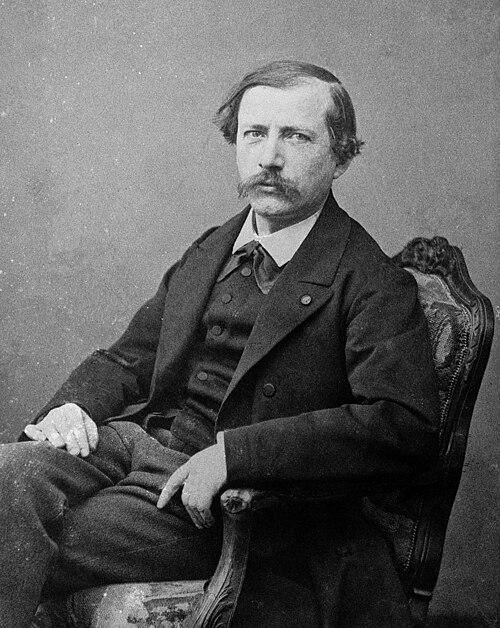
\includegraphics[width=\linewidth]{images/book3/berthelot.jpg}
\end{minipage}\hfill
\begin{minipage}[t]{0.76\linewidth}\vspace{0pt}
मार्सलैं बर्थलो (1827--1907) ने कार्बनिक यौगिकों को प्लैटिनम की परत वाले
इस्पात के बंद पात्र के भीतर संपीडित ऑक्सीजन में जलाया, ताकि
दहन पूर्ण हो और कुछ भी बाहर न निकले: यही ऊष्मामितीय बम है, जो आज भी
दहन ऊष्माओं का प्रामाणिक उपकरण है। उन्होंने ``\omterm{def:b2:reaction-enthalpy:exothermic}{ऊष्माक्षेपी}'' और ``\omterm{def:b2:reaction-enthalpy:exothermic}{ऊष्माशोषी}''
के मूल शब्द भी गढ़े। (छायाचित्र: सार्वजनिक अधिकार-क्षेत्र, विकिमीडिया
कॉमन्स।)
\end{minipage}
\end{history}

\section{अभ्यास}

\begin{exercise}[$\star$]\label{exo:b2:reaction-enthalpy:1}
अध्याय की \omterm{def:b2:reaction-enthalpy:formation}{मानक संभवन एन्थैल्पियों} का उपयोग करके प्रोपेन के दहन
\ce{C3H8(g) + 5O2(g) -> 3CO2(g) + 4H2O(l)} का \qty{298}{K} पर
$\Delta_r H^\circ$ परिकलित कीजिए, जबकि $\Delta_f
H^\circ(\ce{C3H8}, \text{g}) = \qty{-104.7}{kJ/mol}$ दिया है। क्या अभिक्रिया
\omterm{def:b2:reaction-enthalpy:exothermic}{ऊष्माक्षेपी} है?
% ledger: dfh:C3H8_g
\end{exercise}

\begin{exercise}[$\star$]\label{exo:b2:reaction-enthalpy:2}
\qty{1.00}{kg} मेथेन (बनने वाला जल द्रव) और \qty{1.00}{kg} डाइहाइड्रोजन,
\ce{H2(g) + 1/2O2(g) ->
H2O(l)}, को जलाने पर मुक्त ऊष्मा परिकलित कीजिए। कौन-सा ईंधन प्रति किलोग्राम अधिक ऊष्मा देता है?
\end{exercise}

\begin{exercise}[$\star$]\label{exo:b2:reaction-enthalpy:3}
बम कैलोरीमीटर \qty{298}{K} पर \ce{C6H6(l) + 15/2O2(g) -> 6CO2(g) + 3H2O(l)}
के रूप में जलने वाली द्रव बेन्ज़ीन के लिए $\Delta_r U = \qty{-3264}{kJ/mol}$
देता है। $\Delta_r H$ परिकलित कीजिए।
\end{exercise}

\begin{exercise}[$\star$]\label{exo:b2:reaction-enthalpy:4}
\ce{C(s) + O2(g) ->
CO2(g)} के लिए $\Delta_r H^\circ = \qty{-393.5}{kJ/mol}$ और \ce{CO(g) +
1/2O2(g) -> CO2(g)} के लिए $\Delta_r H^\circ = \qty{-283.0}{kJ/mol}$ दिए होने पर, \ce{CO2(g) + C(s) -> 2CO(g)} की एन्थैल्पी परिकलित कीजिए,
जो वात्या भट्ठी के गर्म कोक में होने वाली अभिक्रिया है।
\end{exercise}

\begin{exercise}[$\star\star$]\label{exo:b2:reaction-enthalpy:5}
C--Cl के लिए \qty{350}{kJ/mol} लेकर, अध्याय की आबंध एन्थैल्पियों से
\ce{CH4(g) + Cl2(g) -> CH3Cl(g) + HCl(g)} की एन्थैल्पी का आकलन कीजिए।
फिर, $\Delta_f H^\circ(\ce{CH3Cl}, \text{g}) = \qty{-83.7}{kJ/mol}$ दिया होने पर,
यही राशि संभवन एन्थैल्पियों से परिकलित कीजिए, और अंतर पर
टिप्पणी कीजिए।
% ledger: dfh:CH3Cl_g
\end{exercise}

\begin{exercise}[$\star\star$]\label{exo:b2:reaction-enthalpy:6}
\qty{298}{K} पर जल की मानक वाष्पन एन्थैल्पी
$\Delta_f H^\circ(\ce{H2O}, \text{g}) - \Delta_f H^\circ(\ce{H2O},
\text{l})$ है। इसे परिकलित कीजिए। द्रव के लिए $C_{p,m}^\circ = \qty{75.35}{J/(K.mol)}$ और
वाष्प के लिए \qty{33.59}{J/(K.mol)} लेकर, दोनों को स्थिर मानते हुए,
\qty{400}{K} (दाब के अधीन अतितप्त जल) पर इसका आकलन कीजिए,
और सारणियों से तुलना कीजिए, जो \qty{400}{K} पर द्रव के लिए $\Delta_f H^\circ =
\qty{-282.59}{kJ/mol}$ और वाष्प के लिए \qty{-242.85}{kJ/mol}
देती हैं।
% ledger: cp:H2O_l.298, cp:H2O_g.298, janafdfH:H2O_l.400, janafdfH:H2O_g.400
\end{exercise}

\begin{exercise}[$\star\star$]\label{exo:b2:reaction-enthalpy:7}
इन आँकड़ों से बॉर्न--हाबर चक्र द्वारा पोटैशियम क्लोराइड की \omterm{def:b2:reaction-enthalpy:lattice-enthalpy}{जालक एन्थैल्पी}
परिकलित कीजिए: $\Delta_f H^\circ(\ce{KCl}, \text{s}) = \qty{-436.7}{kJ/mol}$,
पोटैशियम का ऊर्ध्वपातन \qty{89.0}{kJ/mol}, पोटैशियम की आयनन ऊर्जा
\qty{4.341}{eV}, $\Delta_f H^\circ(\ce{Cl}, \text{g}) =
\qty{121.3}{kJ/mol}$, क्लोरीन की इलेक्ट्रॉन बंधुता \qty{3.613}{eV}। यह
सोडियम क्लोराइड की \omterm{def:b2:reaction-enthalpy:lattice-enthalpy}{जालक एन्थैल्पी} से छोटी क्यों है?
% ledger: dfh:KCl_cr, dfh:K_g, ie:K, janaf:Cl, ea:Cl
\end{exercise}

\begin{exercise}[$\star\star$]\label{exo:b2:reaction-enthalpy:8}
एक कॉफ़ी-कप कैलोरीमीटर का अंशांकन \qty{2.00}{kJ} विद्युत ऊर्जा
प्रवाहित करके किया जाता है, जिससे उसका ताप \qty{0.418}{K} बढ़ता है। फिर
उसमें \qty{1.00}{mol/L} के \qty{50.0}{mL} हाइड्रोक्लोरिक अम्ल को
\qty{1.10}{mol/L} के \qty{50.0}{mL} सोडियम हाइड्रॉक्साइड विलयन के साथ मिलाया जाता है,
दोनों एक ही प्रारंभिक ताप पर: ताप \qty{0.583}{K} बढ़ता है।
\ce{H3O+(aq) + OH-(aq) ->
2H2O(l)} की एन्थैल्पी परिकलित कीजिए।
\end{exercise}

\begin{exercise}[$\star\star$]\label{exo:b2:reaction-enthalpy:9}
पेट्रोल का एक मॉडल, ऑक्टेन, $\Delta_f H^\circ(\text{l}) =
\qty{-250.3}{kJ/mol}$ रखता है। उसके दहन की एन्थैल्पी (जल
द्रव), प्रति किलोग्राम मुक्त ऊष्मा, और प्रति मेगाजूल उत्सर्जित कार्बन
डाइऑक्साइड का द्रव्यमान परिकलित कीजिए। मेथेन से तुलना कीजिए।
% ledger: dfh:C8H18
\end{exercise}

\begin{exercise}[$\star\star\star$]\label{exo:b2:reaction-enthalpy:10}
शुद्ध ऑक्सीजन की रससमीकरणमितीय मात्रा में जलती मेथेन का \omterm{def:b2:reaction-enthalpy:flame-temperature}{रुद्धोष्म ज्वाला ताप},
स्थिर ऊष्मा धारिताओं के साथ (अध्याय की
\qty{298}{K} वाली: \ce{CO2} 37.13, \ce{H2O(g)}
\qty{33.59}{J/(K.mol)}), परिकलित कीजिए। इसी सन्निकटन में वायु वाले परिणाम,
\qty{2780}{K}, से तुलना कीजिए। ऑक्सीजन में वास्तविक ज्वाला इस
परिकलन के कथन से कहीं ठंडी क्यों होती है?
% ledger: cp:CO2_g.298, cp:H2O_g.298
\end{exercise}

\begin{exercise}[$\star\star\star$]\label{exo:b2:reaction-enthalpy:11}
किसी गैस की ऊष्मा धारिता प्रायः $C_{p,m}^\circ = a + bT$ लिखी जाती है।
अमोनिया के संश्लेषण के लिए $\Delta_r a = \qty{-60.5}{J/(K.mol)}$ और
$\Delta_r b = \qty{0.0540}{J/(K^2.mol)}$ लीजिए (\qty{300}{K} और \qty{800}{K}
के बीच सारणियों पर समंजित)। \omterm{thm:b2:reaction-enthalpy:kirchhoff}{किरखॉफ़ के नियम} का
\qty{298}{K} से \qty{700}{K} तक समाकलन कीजिए और सारणियों के मान,
\qty{-105.2}{kJ/mol}, तथा स्थिर-$C_p$ आकलन से तुलना कीजिए।
\end{exercise}

\begin{exercise}[$\star\star\star$]\label{exo:b2:reaction-enthalpy:12}
इंजनों में नाइट्रोजन मोनॉक्साइड \ce{N2(g) + O2(g) -> 2NO(g)} द्वारा बनती है।
\qty{298}{K} पर इसकी \omterm{def:b2:reaction-enthalpy:standard-reaction-enthalpy}{मानक अभिक्रिया एन्थैल्पी} परिकलित कीजिए। दिखाइए कि यदि
$\Delta_r C_p^\circ$ छोटा हो, तो अभिक्रिया \qty{2000}{K} पर लगभग उतनी ही
ऊष्मा अवशोषित करती है; \qty{298}{K} पर सारणियों की ऊष्मा धारिताओं से
(\ce{NO} \qty{29.85}{J/(K.mol)}, \ce{N2} 29.12, \ce{O2}
\qty{29.38}{J/(K.mol)}),
\qty{298}{K} और \qty{2000}{K} के बीच परिवर्तन का आकलन कीजिए। समझाइए कि कोई \omterm{def:b2:reaction-enthalpy:exothermic}{ऊष्माशोषी}
अभिक्रिया ठीक सबसे गर्म ज्वालाओं में ही समस्या क्यों बन सकती है।
% ledger: dfh:NO_g, cp:NO_g.298, cp:N2_g.298, cp:O2_g.298
\end{exercise}

\section{समस्या: कैंपिंग-गैस का कारतूस}

\begin{problem}[{सप्ताहांत समस्या --- ब्यूटेन की ऊर्जा, बम कैलोरीमीटर में
एक मापन, बर्तन में गर्म किया गया पानी, और ज्वाला का
ताप}]
\label{pb:b2:reaction-enthalpy:1}
एक कैंपिंग स्टोव \qty{230}{g} वाले कारतूस की ब्यूटेन जलाता है।
\qty{298}{K} पर आँकड़े ($\Delta_f H^\circ$, \unit{kJ/mol} में): \ce{C4H10(g)}
$-125.6$, \ce{CO2(g)} $-393.51$, \ce{H2O(l)} $-285.83$, \ce{H2O(g)}
$-241.83$। मोलर द्रव्यमान: \ce{C4H10} \qty{58.12}{g/mol}, \ce{H2O}
\qty{18.02}{g/mol}। द्रव जल की ऊष्मा धारिता
\qty{75.35}{J/(K.mol)}। शुष्क वायु, आयतन के अनुसार: \qty{20.95}{\percent} \ce{O2},
\qty{78.08}{\percent} \ce{N2}, \qty{0.93}{\percent} \ce{Ar}। $R = \qty{8.314}{J/(K.mol)}$।
% ledger: dfh:C4H10_g, dfh:CO2, dfh:H2O-l, dfh:H2O_g, cp:H2O_l.298, air:O2, air:N2, air:Ar

\medskip
\noindent\textbf{भाग I --- ईंधन।}
\begin{enumerate}
  \item एक मोल ब्यूटेन के लिए, बनने वाले जल को द्रव मानकर, ब्यूटेन का
        पूर्ण दहन लिखिए।
  \item \qty{298}{K} पर इसकी \omterm{def:b2:reaction-enthalpy:standard-reaction-enthalpy}{मानक अभिक्रिया एन्थैल्पी} परिकलित कीजिए।
  \item जल को वाष्प के रूप में बनता मानकर इसे फिर परिकलित कीजिए, और
        अंतर समझाइए।
  \item दोनों स्थितियों में प्रति ग्राम ब्यूटेन मुक्त ऊष्मा परिकलित कीजिए।
  \item इन दोनों मानों में से कौन-सा कैंपिंग स्टोव का वर्णन करता है, जिसका जल
        वाष्प के रूप में ज्वाला से निकलता है?
  \item पूरा कारतूस स्टोव पर कितनी ऊष्मा मुक्त कर सकता है?
\end{enumerate}

\medskip
\noindent\textbf{भाग II --- एक मापन।}
\qty{0.500}{g} ब्यूटेन का एक नमूना ऐसे बम कैलोरीमीटर में जलाया जाता है जिसकी
ऊष्मा धारिता \qty{10.00}{kJ/K} है; बनने वाला जल संघनित हो जाता है।
\begin{enumerate}[resume]
  \item बम कैलोरीमीटर कौन-सी राशि मापता है, और क्यों?
  \item प्रश्न 1 की अभिक्रिया का $\Delta\nu_{\text{गैस}}$ परिकलित कीजिए।
  \item अपेक्षित $\Delta_r U$ परिकलित कीजिए।
  \item कैलोरीमीटर की अपेक्षित ताप-वृद्धि परिकलित कीजिए।
  \item पढ़ी गई वृद्धि \qty{2.461}{K} है। मापे गए $\Delta_r U$
        और $\Delta_r H$, तथा सारणियों से आपेक्षिक अंतर निकालिए।
\end{enumerate}

\medskip
\noindent\textbf{भाग III --- बर्तन।}
\begin{enumerate}[resume]
  \item \qty{1.00}{L} जल
        (\qty{1.00}{kg}) को \qty{20}{\celsius} से \qty{100}{\celsius} तक लाने के लिए आवश्यक ऊष्मा परिकलित कीजिए।
  \item स्टोव यह काम \qty{16.0}{g} ब्यूटेन से करता है। उसकी
        दक्षता (जल द्वारा प्राप्त ऊष्मा बटा मुक्त ऊष्मा) परिकलित कीजिए।
  \item शेष ऊष्मा कहाँ जाती है?
  \item इस दक्षता पर पूरा कारतूस कितने लीटर जल को उबाल तक
        ला सकता है?
\end{enumerate}

\medskip
\noindent\textbf{भाग IV --- ज्वाला।}
\begin{enumerate}[resume]
  \item ब्यूटेन वायु की रससमीकरणमितीय मात्रा में जलती है। एक मोल ब्यूटेन
        के लिए आवश्यक डाइऑक्सीजन के साथ आने वाली डाइनाइट्रोजन और आर्गन की
        मात्राएँ परिकलित कीजिए।
  \item नाइट्रोजन और आर्गन सहित, उत्पादों की मात्राएँ सूचीबद्ध कीजिए।
  \item दो चरणों वाले पथ से समझाइए कि
        \qty{298}{K} पर अभिक्रिया द्वारा मुक्त ऊष्मा (जल वाष्प के रूप में) पूरी की पूरी इन गैसों को
        गर्म करने में क्यों लगती है।
  \item \qty{298}{K} की ऊष्मा धारिताओं, \ce{CO2} 37.13,
        \ce{H2O(g)} 33.59, \ce{N2} 29.12, \ce{Ar} \qty{20.79}{J/(K.mol)}, से
        उत्पादों की ऊष्मा धारिता परिकलित कीजिए।
  \item स्थिर ऊष्मा धारिताओं के साथ ज्वाला का ताप निकालिए।
  \item सारणियों की एन्थैल्पी वृद्धियाँ, एक मोल ब्यूटेन के उत्पादों के लिए,
        \qty{298}{K} और \qty{2300}{K} के बीच \qty{2515.7}{kJ}, और
        \qty{298}{K} और \qty{2400}{K} के बीच \qty{2655.7}{kJ} देती हैं।
        रैखिक अंतर्वेशन से ज्वाला का ताप ज्ञात कीजिए।
  \item पहला आकलन बहुत ऊँचा क्यों है?
  \item ब्यूटेन ज्वाला का मापा गया ताप उससे भी कम क्यों है?
  \item वायु में ब्यूटेन का \omterm{def:b2:reaction-enthalpy:flame-temperature}{रुद्धोष्म ज्वाला ताप} बताइए।
\end{enumerate}
\end{problem}
